\documentclass{cta-author}
\usepackage{listings}
\usepackage{algorithm2e}
\usepackage[]{amsmath}
\usepackage{amssymb}
\usepackage{pifont}
\newtheorem{theorem}{Theorem}{}
\newtheorem{corollary}{Corollary}{}
\newtheorem{remark}{Remark}{}
\usepackage[utf8]{inputenc}

\newcommand{\prototype}{\textsc{Breacher} }
\newcommand{\cmark}{\ding{51}}%
\newcommand{\xmark}{\ding{55}}%

\usepackage{xcolor}
\usepackage{textcomp}

\definecolor{comment}{RGB}{0,128,0} % dark green
\definecolor{string}{RGB}{255,0,0}  % red
\definecolor{keyword}{RGB}{0,0,255} % blue

\lstdefinestyle{c}{
	commentstyle=\color{comment},
	stringstyle=\color{string},
	keywordstyle=\color{keyword},
	%basicstyle=\footnotesize\ttfamily,
	basicstyle=\linespread{0.7}\ttfamily\footnotesize,
	numbers=left,
	numberstyle=\ttfamily,
	numbersep=5pt,
	frame=lines,
	breaklines=true,
	prebreak=\raisebox{0ex}[0ex][0ex]{\ensuremath{\hookleftarrow}},
	showstringspaces=false,
	upquote=true,
	tabsize=1,
	columns=fullflexible,
	%	linespread=0.8,
}

\begin{document}

\supertitle{Submission Template for IET Research Journal Papers}

\title{Discover Deeper Bugs with Dynamic Symbolic Execution 
	and Coverage-based Fuzz Testing}

\author{\au{Bin Zhang$^{1,2\corr}$}, 
	\au{Chao Feng$^{1}$}, 
	\au{Adrian Herrera$^2$}, 
	\au{Vitaly Chipounov$^3$}, 
	\au{George Candea$^2$}, 
	\au{Chaojing Tang$^{1}$}}
%
\address{\add{1}{School of Electronic Science and Engineering, 
		National University of Defense Technology (NUDT), 
		Changsha, Hunan, P.R.China}
\add{2}{School of Computer and Communication Sciences, 
	École Polytechnique Fédérale de Lausanne (EPFL),
	 Lausanne, Switzerland}
\add{3}{Cyberhaven, Inc., 401 Park Drive, Suite 811 Boston, 
	MA 02215, USA}
\email{bizh4ng@hotmail.com}}

\begin{abstract}
Coverage-based fuzz testing and dynamic symbolic execution are both 
popular program testing techniques. However, on their own, both techniques 
suffer from scalability problems when considering the complexity of 
modern software. Hybrid testing methods attempt to mitigate these 
problems by leveraging dynamic symbolic execution to assist fuzz 
testing. Unfortunately, the efficiency of such methods is still 
limited by specific program structures and the schedule of seed files.

In this paper, we introduce a novel lazy symbolic pointer concretization 
method and a symbolic loop bucket optimization to mitigate path explosion 
caused by dynamic symbolic execution in hybrid testing.
We also propose a distance-based seed selection method to rearrange the 
seed queue of the fuzzer engine in order to achieve higher coverage. We implemented 
a prototype and evaluate its ability to find vulnerabilities in software 
and cover new execution paths. We show on different benchmarks that 
it can find more crashes than other off-the-shelf vulnerability 
detection tools. We also show that our method can discover 43\% more 
unique paths than vanilla fuzz testing.
\end{abstract}

\maketitle

\section{Introduction} \label{sec:introduction}
Fuzz testing is a popular technique for automatic software
vulnerability detection \cite{Miller:Fuzz, 5010257, sutton2007fuzzing},
but suffers from low efficiency when applied to real-world software
\cite{neystadt2008automated, godefroid2008automating, ganesh2009taint,
	cadar2011symbolic, rawat2017vuzzer, stephens2016driller}. Software
often parses complex input formats such as PDF, DOCX, or JPEG, which
generates deep execution paths with complex conditions. Traditional
random fuzzers generate shallow test cases because they are unable to
guess the inputs that would help reach deeper parts of the code. More
sophisticated fuzzers discard test inputs that do not add new coverage
and keep the remaining inputs in a seed file queue. They then derive
new test input from the seed queue using genetic algorithms
\cite{rawat2017vuzzer, online:afl, stephens2016driller}. Although
coverage-based fuzz testing is able to discover more paths than
traditional fuzz testing, it is nevertheless incapable of triggering
bugs that are deeply nested in complex code areas, due to the random
nature of the mutations.

Dynamic symbolic execution alleviates some of the challenges
encountered by fuzzers. Whereas fuzzers try millions of different
concrete inputs (e.g., "abc", 1, ...) in order to reach deeper parts of
the code, symbolic execution uses symbolic inputs (e.g., $\lambda$)
that concisely summarize all possible concrete values (e.g., all values
of a 32-bit integer). When a symbolic value reaches a branch condition,
the symbolic execution engine invokes a constraint solver in order to
compute the exact value that would drive the program down the desired
path. Unfortunately, pure symbolic execution often results in an
exponential number of paths that bottlenecks the constraint solver.

Recent work aims to combine the advantages of symbolic execution and
fuzz testing. In this hybrid approach~\cite{godefroid2012sage,
	yeh2015craxfuzz, majumdar2007hybrid, pak2012hybrid}, corner cases that
are difficult for fuzzers to cover are generated from dynamic symbolic
execution by solving the corresponding path constraints. Conversely,
dynamic symbolic execution also benefits from the fuzzer-generated
seeds in order to quickly reach more code areas without getting lost in
a large execution tree. Driller, which is built on top of the Angr
symbolic execution engine \cite{Shoshitaishvili_firmalice-automatic},
and the AFL fuzzing engine \cite{online:afl}, have attempted to
leverage symbolic execution to solve the branches guarded by complex
path conditions to avoid saturation of fuzzer
\cite{stephens2016driller}. Driller's performance in DARPA's Cyber
Grand Challenge (CGC) \cite{online:CGC} demonstrates the potential of
these hybrid testing approaches.

In hybrid testing, such as Driller, the performance gain from dynamic
symbolic execution is still limited by particular program
structures, such as symbolic pointers and loops~\cite{schwartz2010all,
	Boonstoppel:RAP, cadar2011symbolic, baldoni2016survey}. These structures
quickly generate many redundant paths that do not trigger new behaviors
but result in \textit{path explosion}. This is compounded by the possibly
large number of seed files generated by the fuzzer.

This paper makes three main contributions. We propose three new
techniques to improve the efficiency of hybrid testing. First, we
improve the lazy concretization of symbolic pointers presented
in~\cite{chipounov2011s2e}. Second, we enhance the AFL's loop bucketing
technique~\cite{online:afl} in order to avoid getting stuck in loops
that have a symbolic iteration counter. Third, in order to address the
large size of the seed queue, we propose a distance-based seed
selection algorithm in order to improve coverage when testing time is
limited. Each seed in the queue is weighted by runtime information, i.e.,
path and memory coverage, then the seed with greater weight is assigned with
more mutation times. We also 
implemented our prototype \prototype and benchmarked it on 
(1) a sample program that contains 9
different types of representative bugs, (2) the LAVA benchmark suite
\cite{dolan2016lava}. 
The experiments show that \prototype triggers more bugs
than other state-of-the-art vulnerability detection tools. 
The evaluation results on several real-world programs show that our approach can
discover 43\% more unique paths on average than traditional random fuzz
testing. Also, \prototype exposed several unreported crashes in real-world programs. 

The rest of this paper is organized as follows.
Section~\ref{sec:preliminaries} introduces dynamic symbolic execution
and hybrid testing. Section~\ref{sec:ease PE} presents the details of
how we deal with \textit{path explosion} caused by symbolic pointers
and loops. Section~\ref{sec:seed selection} presents the distance-based
seed selection algorithm. Section~\ref{sec:evaluate} describes the
implementation of \prototype and the evaluation results.
Section~\ref{sec:discussion} discusses the limitations of our work and
possible further research topics. Finally, Section~\ref{sec:related} reviews
related work and Section~\ref{sec:conclusion} concludes the paper.


\section{Preliminaries} \label{sec:preliminaries}
%Preliminaries of symbolic execution and hybrid testing

In this section, we first review the theoretical foundation of dynamic
symbolic execution. Then we provide a simple example in
Listing~\ref{PRE} to illustrate the concept of hybrid testing based on
fuzz testing and dynamic symbolic execution.

\subsection{Dynamic Symbolic Execution}

Symbolic execution is an analysis method to determine what input can
drive execution to specific code regions \cite{King:Symbex}. It
interprets the program by assigning \textit{symbolic data} rather than
actual (\textit{concrete}) data to the program inputs.

Consider a program $P$ which consists of a set of program variables
$Var$ and a set of instructions $Inst$. 
An \textbf{\textit{execution path}} is a serial of instructions, such as 
$I_0\rightarrow I_1 \rightarrow \cdots\rightarrow I_n$, where $I_i\in Inst$.
Unlike execution path, which focuses on instructions, a 
\textbf{\textit{program state}} describes current execution state, which
holds the value of each variable (a variable 
can be represented by either register or memory).
Since the bits of register and memory are bounded, the number of program
state can be enumerated. However, the total number of execution path 
may be infinite, which is also known as ``path explosion'' problem.

Dynamic symbolic execution
maintains a \textbf{\textit{symbolic state}} 
$\mathcal{S}=\langle I,M,S,pc\rangle$, where 
$I\in Inst$ denotes the next instruction to be executed, 
$M$ is the concrete memory store which maps $Var$ to concrete data, 
$S$ is the symbolic memory store which maps $Var$ to symbolic expressions, 
and $pc$ is the symbolic path constraint which is a first order 
quantifier free formula over symbolic expressions. Since each symbolic state 
can be individually mapped to an execution path, we can use \textit{symbolic state} 
to equivalently represent an execution path.
In the following sections of this paper, all \textit{states} 
denote the \textit{symbolic state} unless explicitly stated. 
And the ``path explosion'' problem can also be expressed as ``state explosion''.

Under dynamic symbolic execution, program $P$ operates on both concrete
memory $M$ and symbolic memory $S$ by executing each instruction $I\in
Inst$. The semantics for different types of instructions are listed in
Table~\ref{table:DSE-inst}.

\begin{table}[!b]
	\processtable{Instructions in dynamic symbolic execution, as well as
		their expressions and semantics.\label{table:DSE-inst}}
	{\begin{tabular*}{20pc}{@{\extracolsep{\fill}}lcl@{}}\toprule
			Type  & Expression & Semantic\\
			\midrule
			Assignment   &  $v:=e$ & Update $v$ with expression $e$\\
			Terminate    &  abort/exit & Terminate current state \\
			Conditional  &  \textbf{if} $e$ \textbf{then} $I_{true}$ \textbf{else} $I_{false}$ & Fork current state\\
			\botrule
		\end{tabular*}}{}
	\end{table}
	
The objective of dynamic symbolic execution is to systematically
explore all feasible paths of program $P$ under the initial input.
Consider an input vector $\iota$ which steers program $P$ to execute a
unique finite program trace
$s_0\xrightarrow{I_1}s_1\cdots\xrightarrow{I_n}s_n$, where $I_1\cdots
I_n\in Inst$ and $s_1\cdots s_n$ are program states. Then during the
execution of dynamic symbolic execution, different types of
instructions are handled differently according to their semantics. If
$I_i$ is an assignment instruction $v:=e$, dynamic symbolic execution
updates the symbolic memory of $v$ directly with expression $e$, i.e.,
$S(v):= e$. If $I_i$ is a conditional instruction as defined
previously, any satisfying assignments to the Boolean expression
$pc\wedge e$ will lead $P$ to execute the \textit{then} branch and any
satisfying assignments to Boolean expression $pc\wedge\neg e$ will
steer $P$ to run the \textit{else} branch. Dynamic symbolic execution
tries to explore both \textit{then} and \textit{else} branches
simultaneously by \textit{state forking}. To fork a new state, dynamic
symbolic execution uses a constraint solver $T$ to generate
solutions both for $pc\wedge e$ and $pc\wedge\neg e$ and updates the
path constraints accordingly. By forking new program state for each
executed conditional instruction, all possible path constraints can be
enumerated and eventually all feasible paths in $P$ can be exercised.
Whenever dynamic symbolic execution executes a terminate instruction,
it terminates the current state and employs the constraint solver to
solve the current $pc$ to generate a corresponding \textit{test input}.

Dynamic symbolic execution is affected by the \textit{path explosion}
problem. Since dynamic symbolic execution may fork a new state for
every conditional branch, the number of states may grow exponentially
in the number of conditional instructions~\cite{cadar2013symbolic}. A
large number of states will quickly exhaust computation resources and
halt testing.

\subsection{Hybrid Testing}

The sample program in Listing~\ref{PRE} tries to verify the three input
parameters. Hybrid testing starts from a coverage-based fuzzer which
quickly generates an input that satisfies the \textit{else} branch
of the conditional instruction at line 2. However, verification of
\texttt{checksum} at line 5 would typically prevent the fuzzer from
going any further. When the fuzzer gets stuck, hybrid testing switches to
dynamic symbolic execution engine to get more coverage.

\lstinputlisting[label={PRE}, language=C,style=c,caption={A motivating
	code for preliminaries. Note that all example code in this paper is
	given as source code for readability, but our approach operates
	directly on binary programs.}]{pre.c.tex}

Figure~\ref{s2e-assist} shows the general architecture of a hybrid testing
approach based on fuzz testing and symbolic execution. The fuzzing engine 
performs coverage-based fuzz testing, and shares the already explored 
path information with the symbolic execution engine. This already explored 
path information can be recorded in any forms. For example, AFL 
intercepts transitions between basic blocks as well as the branch-taken 
hit counts, and store these information into a \textit{Bitmap}.
Then each test case in the seed queue will be sent to symbolic execution 
engine to disclose more new paths.
Unlike traditional dynamic symbolic execution, the symbolic execution engine
only forks for branches that have not been previously covered. For
example, as shown in Figure~\ref{s2e-assist}, suppose the red execution
trace is the path that the fuzzer will taken. In this case the symbolic
execution engine will only fork new states when it finds uncovered
branches (the blue branches) according to the shared internal
information from the fuzzer. Each forked state will generate a new test
case which can help the fuzzer to reach new code areas. Based on this
hybrid testing method, the verification of \texttt{header->checksum} at
line 5 can be solved by symbolic execution engine and generate a new
test case for further fuzzing.

However, function \texttt{path\_explosion} makes it hard to solve the 
conditional instruction at line 9. For example, when using BFS exploration 
strategy, this function will quickly saturate the symbolic state's number 
budget that used to avoid memory overhead \cite{stephens2016driller}; DFS 
exploration works better than BFS in this example, but it may degrade to 
exhaustive testing in some cases (e.g., when \texttt{path\_explosion} deals
\texttt{flag} as a symbolic pointer). 
We will discuss our mitigation
for this problem in Section~\ref{sec:ease PE}.


\section{Mitigating Path Explosion in \textit{SPF}} \label{sec:ease PE}
Hybrid testing can help to reduce \textit{memory overhead} by 
limiting the number of states to an acceptable level. However, 
as mentioned in Section~\ref{sec:introduction}, symbolic pointers 
and loops will quickly generate lots of useless states that may 
not cover new code areas but bring serious performance overhead.

To address the large number of states forked from symbolic pointers, 
we propose a novel \textit{lazily concretization} of symbolic 
pointers which can not only reduce the number of states but also 
improve coverage. 
For symbolic loops, we introduce an optimization based on AFL's 
\textit{loop bucket} to control forking in symbolic loops. By 
doing this, execution can reach deeper code areas without 
generating lots of states. Both improvements will be discussed 
in the following sections.

\begin{figure}
	\centering
	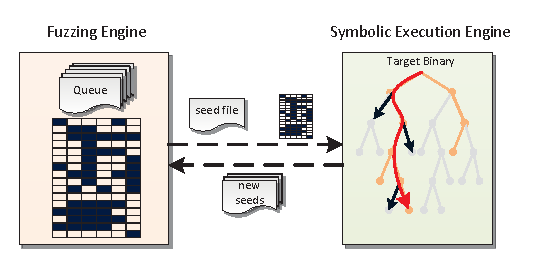
\includegraphics[width=0.5\textwidth]{s2e-assist.eps} 
	\caption{Dynamic symbolic execution assisted fuzz testing. The 
		symbolic execution engine can help generate fresh seeds for 
		the fuzzing engine based on the seed files 	and the already 
		explored path information.}\label{s2e-assist}
\end{figure}

\subsection{Lazy Concretization of Symbolic Pointer}
The code snippet in Listing~\ref{RE-LCSP} shows the basic symbolic pointer 
problem in dynamic symbolic execution. The first parameter 
(i.e., \texttt{buf}) of function \texttt{looks\_ascii} points to memory 
that contains symbolic input data. The \texttt{nbytes} parameter is a 
concrete value that denotes the size of the memory buffer pointed by 
\texttt{buf}. \texttt{ubuf} is a shadow buffer which is used for further 
processing. 
Function \texttt{looks\_ascii} tries to determine whether each character 
of the symbolic input data appears in plain ASCII text, and returns 
immediately once a non-plain ASCII text character appears. 
The symbolic execution engine faces the symbolic pointer problem when executing 
the code at line 18 because \texttt{buf[i]} is from the symbolic input data. 
The memory range of \texttt{text\_chars[buf[i]]} spans from \texttt{\&text\_chars} 
to \texttt{\&text\_chars+255}. Since the binary executable loses the 
type information, the symbolic execution engine may need to explore all 256 possible
values for each \texttt{buf[i]} at the worst case. Meanwhile, the loop from line
17 to line 22 makes the trigger of the bug at line 26 even harder since more
states will be forked when \texttt{nbytes} is a larger one.

There are different approaches for handling path explosion caused by
symbolic pointers. For example, treating memory address as \textbf{fully symbolic} 
enables the executor to reason about all possible values for symbolic pointer
\cite{song2008bitblaze, thakur2010directed, brumley2011bap, trtik2014symbolic}.
This can be achieved by either forking states or employing nested 
\textit{if-then-else} formulas which encode all possible values. 
However, since a symbolic address may pointer to any memory cell, fully symbolic
memory model fails to scale for real-world binary software. 
Some researches leverage the \textit{theories of arrays} to make fully symbolic 
memory model scalable \cite{cadar2006exe}\cite{cadar2008klee}. 
For example, KLEE \cite{cadar2008klee} forks states for values that reference 
different objects, and the \textit{theories of arrays} is leveraged within the same object.
However, since our target is to analyze binary executable whose object size of data structure is 
unavailable, the number of objects increases because each possible value may reference to a 
different object.
In contrast to reason about all possible values, a \textbf{partial symbolic} memory model has been proposed \cite{cha2012unleashing, avgerinos2014exploiting, Shoshitaishvili_firmalice-automatic}.  
The partial symbolic memory model tries to concretize all symbolic pointer write 
operation and treats symbolic pointer read operation using a fully 
symbolic memory model when contiguous interval of possible values is small enough.
However, if the possible values spans a large area, partial symbolic memory model
still needs to concretize the symbolic pointer which may lose some soundness paths.

The \textit{lazy forking} strategy leveraged in S2E was proposed to avoid 
maintaining expensive symbolic pointers and ease the large number 
of states by forking \textit{pending states} in concolic 
execution \cite{chipounov2011s2e}. 
Consider a memory dereference instruction $I\in Inst$ in program $P$, 
suppose $I$ tries to access memory indexed by a symbolic expression 
$e_{addr}$.
Lazy forking treats such instruction $I$ as a conditional instruction 
and forks new states for $I$. It first evaluates the concrete value 
as $c_{addr}$, then it constructs an equal
expression $condition:= EQ(e_{addr}, c_{addr})$ 
which points $e_{addr}$ to this concrete value. Then it forks a 
new state $s_p=fork(s, ^\neg condition)$ which is labeled as a 
``pending state''. After that, each possible value of $e_{addr}$ 
will be exercised by systematically repeating this process. Even 
though lazy forking still needs to enumerate all possible values, 
it can avoid overhead by significantly reducing the total number 
of states that simultaneously exist in system. Here, 
the $condition$ is called a \textit{hard constraint} and 
$^\neg condition$ is called a \textit{soft constraint}.

For example, for the memory dereference instruction at line 18 
in Listing~\ref{RE-LCSP}, suppose the concrete value of 
\texttt{buf[i]} for $i\in[0,1,2,3]$ is `\texttt{A}'. 
In this case lazy forking will fork a new pending state and 
add the soft constraint $\texttt{buf[i]}\neq\texttt{`A'}$ to 
it. Meanwhile, the path constraint of the original state will 
be appended with the hard constraint $\texttt{buf[i]}=\texttt{`A'}$.
By doing this, the ``path explosion'' problem is postponed to a later moment.

However, the hard constraint may reduce the suffix feasible paths 
to a very small group. For example, suppose the address of a symbolic 
pointer can be expressed as $e_{addr}=f(v_1, v_2,\cdots, v_n)$, 
where $v_1, v_2,\cdots, v_n\in Var$ are variables of program $P$. 
Then expression $condition:= EQ(e_{addr}, c_{addr})$ will limit 
the current execution path only feasible when ($v_1, v_2,\cdots, v_n$) 
equals to ($c_1, c_2,\cdots, c_n$), where $c_i$ are the 
corresponding concrete values. 
Take the sample code in Listing~\ref{RE-LCSP}. The execution path 
to line 26 will be infeasible because the hard constraint limits 
the value of \texttt{buf[i]} ($i\in[0,1,2,3]$) to `\texttt{A}'. 
And the crash can only be triggered after enumerating all possible 
values for \texttt{buf[i]} ($i\in[0,1,2,3]$) in the worst case since
lazy forking still belongs to DFS state exploration strategy.
So even though lazy forking can ease the path explosion problem, 
it may still need to take longer time to trigger interesting paths. 
This will result in performance loss, because the symbolic 
execution engine may hold up the fuzzer. 

To mitigate this problem, we introduce a novel method 
\emph{lazy concretization of symbolic pointer} (LCSP) 
which is built on top of lazy forking. The detailed algorithm 
of LCSP is shown in Algorithm~\ref{LCSP}.


\lstinputlisting[label={RE-LCSP}, language=C,style=c,caption={A 
	motivating code derived from \texttt{file} in GNU Coreutils that contains symbolic pointer dereference at line 18.}, 
float=tp]{real-eaxmple-LSP.c.tex} 

Whenever the execution engine touches a symbolic pointer $e_{addr}$, it obtains 
the range of all possible values $\mathcal{R}$ by invoking function \texttt{getRange} 
in the constraint solver. Then all memory values within the range are dissolved
into buckets $\mathcal{B}=\langle v, addr\rangle$, where $v$ is the memory value; $addr$
is the set of memory cell's address whose memory value is $v$.
After this, we reuse S2E's lazy forking method to pickup 
the bucket that contains the concrete value of this symbolic pointer.
For example, when executing the code at line 18 in Listing~\ref{RE-LCSP}, the range of 
the symbolic pointer is $\mathcal{R}=\texttt{\&text\_chars}+\{0, 1,\cdots, 255\}$.
By scanning the memory cells within $\mathcal{R}$, we can build 4 buckets, i.e., 

$\mathcal{B}_0:\{v=\texttt{F}| addr=[0,1,2,3,4,5,6,\cdots]+\texttt{\&text\_chars}\}$

$\mathcal{B}_1:\{v=\texttt{T}| addr=[7,8,9,10,12,13,\cdots]+\texttt{\&text\_chars}\}$

$\mathcal{B}_2:\{v=\texttt{I}| addr=[160,161\cdots,254,255]+\texttt{\&text\_chars}\}$

$\mathcal{B}_3:\{v=\texttt{X}| addr=[128,129,130,\cdots,159]+\texttt{\&text\_chars}\}$

Since $e_{addr}$'s concrete value belongs to $\mathcal{B}_1$, we then
introduce a new symbolic variable $v_p$ into the engine and update current path constraint by adding expanded hard constraint $condition$ to it. 
$condition$ is descried as $P_v\cap P_p$, where

%$P_\mathcal{B}=\{\bigcup\limits_{i=0}^{Len_{addr}-1}e_{addr}=addr_i\}$;

$P_v=\{v_p=1\}$; 

$P_p=\{e_{addr}=\&\texttt{text\_chars}+0x41\}$.

During the following execution, all path conditions that related to the newly
introduced symbolic variable $v_p$ will be collected as pointer dereference constraint
$C_{pd}$.
This constraint is used to keep execution consistency.

\begin{algorithm}
	\LinesNumbered
	\caption{Lazy concretization of symbolic pointer}
	\label{LCSP}
	\KwIn{Current state $S$, pending states $S_P$, failed condition $C_F$, 
		the set of hard constraints $S_{C_H}$, pointer dereference constraint $C_{pd}$.}
	\KwOut{Testcase $t_{lsp}$ if success.}
	% ignore cases that unrelated to symbolic pointer
	\If{$C_F$ \textbf{is not result from symbolic pointer}}
	{
		return $null$\;
	}
	$offs = S$.getInputOffset($C_F$)\;
	$C_H = S_{C_H}$.getRelated($offs$)\;
	% Collect all possible bucket's addr to Solutions
	$extraCond\leftarrow True$\;
	\ForEach{$s_p$ in $S_P$}
	{
		$off_{fork} = s_p$.getInputOffset($s_p$.forkCondition)\;
		\If{$off_{fork}$ not in $offs$}
		{continue\;}
		$\mathcal{B}=s_p$.buckets\;
		$e_{addr} = s_p$.getForkAddr()\;
		% find all satisfied buckets
		$\mathcal{B}_{sat}=s_p$.getSATBuckets($C_{pd}$, $\mathcal{B}$)\;
		
		% sieve real solutions out
		$curExCond\leftarrow False$\;
		\ForEach{$\mathcal{B}$ in $\mathcal{B}_{sat}$}
		{
			\ForEach{$addr$ in $\mathcal{B}$.addr}
			{
				$s_{tmp} = S$.clone()\;
				$s_{tmp}$.getConditions().strip($C_H$)\;
				$s_{tmp}$.addConstraint($C_F$)\;
				$C_{new}\leftarrow \{e_{addr}=addr\}$\;
				$success = s_{tmp}$.evaluate($C_{new}$)\;
				\If{success}
				{$curExCond\leftarrow curExCond\cup C_{new}$\;}
			}
		}
		$extraCond\leftarrow extraCond\cap curExCond$\;
	}
	
	$s_{tmp} = S$.clone()\;
	$s_{tmp}$.getConditions().strip($C_H$)\;
	$s_{tmp}$.getConditions().strip($C_{pd}$)\;
	$s_{tmp}$.addConstraint($extraCond$)\;
	
	$(success, t_{lsp}) = s_{tmp}$.generateTestCase()\;
	\If{$success$}
	{
		return $t_{lsp}$;
	}
	return $null$\;
\end{algorithm}

When performing lazy forking, all the states whose path constraints 
contain the soft constraints will be collected into \emph{Pending States}
as well as the buckets. 
These pending states are grouped by the program variables (e.g., each 
byte in an input file) that affect the corresponding soft constraint. 
They are also ordered along with the execution trace.
Then when the dynamic symbolic execution engine detects an infeasible 
branch due to hard constraints from symbolic pointer (line 1$\sim$3), 
the branch condition $C_F$ will be 
investigated to extract the program variables $offs$ (line 4).



Since we have introduced new symbolic variable when dereferencing a symbolic pointer,
we need to make sure \textbf{all conditions in $C_{pd}$ are satisfied so that the generated
test case can keep execution consistency}.
Line 14 collects all satisfied buckets into $\mathcal{B}_{sat}$. The collect procedure
is light-weight since \texttt{getSATBuckets} only needs to evaluate $C_{pd}$
under each bucket's key (i.e.,$\mathcal{B}.v$).
For each satisfied bucket, real solutions for current $e_{addr}$ are sieved out 
(line 16$\sim$27). This is achieved by evaluating each $addr$ in $\mathcal{B}_{sat}$
(line 21\&22). All $C_{new}$ evaluated as True will be collected together (line 23
$\sim$25). The $\cup$ in line 24 compacts consecutive $addr$s into a range expression.
For example, $\{e_{addr}=4\}$, $\{e_{addr}=5\}$ and $\{e_{addr}=6\}$ will be transformed to
$\{4<=e_{addr}<=6\}$.

By analyzing all pending states that related to $off_{fork}$, 
the final extra condition $extraCond$ is constructed (line 28).
After this, we remove all hard constraints $S_{C_H}$ and $C_{pd}$ from a newly cloned state $s_{tmp}$
from current state and append
the final extra condition to it (line 31$\sim$33). 
The reason why $C_{pd}$ is stripped is because it is already satisfied at line 14.
After appending all related conditions, the dynamic symbolic execution 
engine will try to generate a new test case (line 34), and once the 
generation successes, the test case $t_{lsp}$ will be sent to the 
fuzzer to find more paths.

For the code in Listing~\ref{RE-LCSP}, suppose \texttt{nbytes} is 5. 
Then when dynamic symbolic execution reaches line 24, there will be 
six states in the system: one execution state $S_0$ and five pending 
states ($P_0$, $P_1$, $P_2$, $P_3$, and $P_4$). $P_i$ is forked when 
dereferencing \texttt{buf[$i$]} at line 18. And the pointer dereference
constraint $C_{pd}$ is 
$\{(v_0=\texttt{T})\cap (v_1=\texttt{T})\cap (v_2=\texttt{T})\cap (v_3=\texttt{T})\cap (v_4=\texttt{T})\}$,
where $v_i$ is introduced for each symbolic pointer dereference at
line 18; $S_{C_H}$ is $\{C_{H0}\cap C_{H1}\cap C_{H2}\cap C_{H3}\cap C_{H4}\}$,
where $C_{Hi}$ is $\{v_i=\texttt{T}\cap \texttt{buf[i]=`A'}\}$.

Because of the hard constraint, the four condition instructions at line 24
are infeasible. We pick up the first failed condition 
$C_F=\{\texttt{ubuf[0]==`D'}\}$ to explain how LCSP works in detail.

The fork failure raises because line 18 introduces $\texttt{buf[0]=`A'}$ in $C_{H1}$, which conflicts with condition \texttt{ubuf[0]==`D'}. 
According to Algorithm~\ref{LCSP}, 
LCSP first checks the input offset that results in this infeasible
condition and deals all pending states related to this offset. 
Based on this,
only $P_0$ is chosen to break \texttt{ubuf[0]==`D'}, and the
corresponding $C_H$ and $e_{addr}$ in Algorithm~\ref{LCSP} is $C_{H1}$ and 
\texttt{text\_chars+buf[0]} respectively.

Then all satisfied buckets of $P_0$ are sieved out by evaluating the 
pointer dereference constraint $C_{pd}$. 
There are four buckets for $P_0$ as mentioned before, i.e., $\mathcal{B}_0$, $\mathcal{B}_1$, $\mathcal{B}_2$, and $\mathcal{B}_3$, whose memory value
$v$ is $\mathcal{B}_0.v=\texttt{F}$, $\mathcal{B}_1.v=\texttt{T}$, $\mathcal{B}_2.v=\texttt{I}$, and $\mathcal{B}_3.v=\texttt{X}$ respectively. 
After evaluating all these four buckets, $\mathcal{B}_{sat}=\{\mathcal{B}_1\}$ since
$C_{pd}$ is only satisfied when $v_0 = \mathcal{B}_1.v=\texttt{T}$.

After this, Algorithm~\ref{LCSP} evaluates each $addr$ in $\mathcal{B}_1$ to build the final extra condition (line 16$\sim$27). The final constructed extra
condition $extraCond$ in this example is $\{e_{addr} = \texttt{\&text\_chars+`D'}\}$.
This $extraCond$ keeps not only $C_F$ but also $C_{pd}$ be satisfied.
Then LCSP fixes current path condition by stripping unrelated conditions and adding
$\{e_{addr} = \texttt{\&text\_chars+`D'}\}$ to it, where $e_{addr}$ is \texttt{text\_chars+buf[0]}.

At last, LCSP invokes the constraint solver to 
generate a fresh test case. Here, after breaking condition \texttt{ubuf[0]==`D'}, the 
generated test case $t_{lsp}$ is \texttt{DAAAA}. This test case will be sent to the fuzzer and the
remained three conditions at line 24 will be solved in the same way. Thus, based on this algorithm, we can generate at least one fresh test case 
that satisfies the branch condition whenever a branch is infeasible 
because of lazy forking. 

\subsection{Optimization for Symbolic Loop}
Symbolic loop, whose loop control variable depends on symbolic data, 
is another common cause of path explosion since its loop times may 
range from 0 to infinite theoretically. 
Even though the hybrid testing method can ease path explosion, the 
states forked from a symbolic loop will quickly force the number of 
states to increase to the budget's upper bound. 

\lstinputlisting[label={RE-SLB}, language=C,style=c,caption={A motivating 
	example to demonstrate path explosion raised by symbolic loops.}]
{example-SLB.c.tex} 

The code snippet in Listing~\ref{RE-SLB} demonstrates this problem. 
Function \texttt{verify\_packet} reads the \texttt{length} of the 
raw data from the \texttt{packet} at line 4.
Then from Line 6 to 10, it investigates each bytes in the raw data 
to determine whether there exists the ending descriptor 
(i.e., \texttt{0xFF}) through a loop structure. 
Suppose we have a test case from the seed queue of 
the fuzzer and its \texttt{length} is \texttt{0xAA}, 
then the symbolic loop 
from line 6 to 10 (\texttt{length} is symbolic) 
will result in path explosion.
Because the possible value of \texttt{length} is in the 
range of [0, $2^{32}-1$], $2^{32}$ states will be forked from 
line 6 in the worst case. 
Most of the forked states from line 6 may not contribute 
to any new code coverage but only bring performance overhead.
It is therefore important to also handle symbolic loops. 

AEG \cite{Avgerinos:2014:AEG:2556647.2560219} proposes \emph{loop exhaustion}
search strategy to handle symbolic loops. It tries to execute the loop as many
times as possible. Since it focuses only on maximizing the loop iterations which
may fork lots of states, it thus may stuck the fuzzer from exploring more paths 
in our hybrid testing framework.

A \textit{boundary state prioritization} method has been proposed recently
to ease the path explosion problem due to symbolic loops.
The key idea of this prioritization is to defer the analysis of 
uninteresting states based on the likelihood of a security vulnerability \cite{cab-fuzz}. 
Specifically, it focuses only on three types of states for a symbolic 
loop: \textit{no loop execution}, \textit{single loop execution}, and 
\textit{the largest number of loop executions}.
The author implemented such a strategy within S2E \cite{chipounov2011s2e} 
and produced a vulnerability detection tool \textit{CAB-Fuzz}.
It successfully found 21 undisclosed unique crashes in Windows 7 and 
Windows Server 2008 \cite{cab-fuzz}.

We extend this boundary state prioritization method by integrating it 
with the \emph{Loop Bucket} mechanism employed in AFL \cite{online:afl} 
to achieve better performance on finding vulnerabilities.
AFL utilizes \emph{Loop Bucket} to avoid collecting too many test cases 
which only affect the loop times into the seed queue \cite{online:afl}. 
It groups the loop times into 8 different buckets, i.e., 
[1, 2, 3, 4-7, 8-15, 16-31, 32-127, 128+]. Only changes that occur 
between different buckets will be regarded as new behaviors. 
Based on this idea, we proposed a \textit{Symbolic Loop Bucket} (SLB) 
to handle the symbolic loop when performing hybrid testing. The 
algorithm of SLB is described in Algorithm~\ref{SLB}.

Loops are extracted from the target program by static analysis. 
These loops will be configured in the dynamic symbolic execution 
engine to help it recognize loops in runtime. All the symbolic loops 
can be distinguished from the others by checking whether the loop 
exit condition is affected by symbolic data or not (line 1$\sim$3). 
For the edge belongs to symbolic loop, the uncovered loop buckets 
for this loop will be obtained by analyzing the \textit{Bitmap} 
mentioned before (line 5). 
In already covered loop buckets, the program will loop for one more 
time without forking new state (line 16\&17). Once an uncovered bucket 
is reached, the corresponding test case will be generated and then 
this uncovered bucket will be removed from the uncovered loop buckets 
to avoid generating multiple test cases (line 7$\sim$12). After 
generating test cases for all the uncovered buckets, the loop will 
be prohibited from being executed for more times. This can make sure 
that all the loop buckets will be covered without causing path explosion.

\begin{algorithm}
	\LinesNumbered
	\caption{Symbolic loop bucket.}
	\label{SLB}
	\KwIn{Configured Loops $L$, Current Edge $CE$ and Bitmap $B_p$}
	\KwOut{Generated test cases $t_{slb}$}  
	\If{not $IsaLoopCycleEdge(L,CE)$ or not $IsaSymLoop(CE)$}
	{
		return;
	}
	$loopTimes$ = 1\;
	$UBs$ = $ParseUncoveredBuckets(B_p)$\;
	\While{TRUE}
	{
		\ForEach{$ub$ in $UBs$}
		{
			\If{$loopTimes$ within $ub$}
			{
				$t_{slb}.add(GenerateTestcase())$\;
				$UBs$.$remove(ub)$\;
			}
		}
		\eIf{$UBs$ is $null$}
		{
			return $t_{lsb}$\;
		}{
		$ExecuteOneCycle()$\;
		$loopTimes += 1$\;
	}
}
\end{algorithm}  

For the symbolic loop in Listing~\ref{RE-SLB}. Suppose previous 
test cases have covered the buckets of [1], [2], [3], and [4-7]. 
Then \textit{UBs} at line 5 in Algorithm~\ref{SLB} will consist of 
[8-15], [16-31], [32-127], and [128+]. 
$\textit{loopTimes}=[1, 2, \cdots, 7]$ will not fork any new states 
according to line 15 to 18. Then once the \textit{loopTimes} reaches 
8 which belongs to an uncovered bucket [8-15], the engine forks a 
new state,  generates the corresponding the test case, and removes 
bucket [8-15] from \textit{UBs}. The execution engines will not 
fork new states until \textit{loopTimes} reaches 16, 32 and 128. 
Once all the loop buckets are covered, the forking in this 
symbolic loop will be disabled. It will continue cycling until 
\textit{loopTimes} reaches the concrete value of \texttt{length} 
(i.e., \texttt{0xAA}) and then exercise deeper code areas.

\section{Distance-based Seed Selection} \label{sec:seed selection}
As previously discussed, the size of the fuzzer's seed queue will quickly 
reach a large number (especially with the assistance of dynamic symbolic 
execution) when testing large-scale modern software. The seed queue should 
therefore be rearranged to find more paths in a given time budget.

We realized that different seed files in the queue have different affects 
on path discovery. For example in Figure~\ref{motivate-example}, suppose 
each input that triggers new behavior will be mapped to a specific dot. 
The fuzzer starts from an initial seed which is marked as red in this figure. 
The mutation results of this initial seed cover the black points 
as well as seed A and seed B. Then, in evolutionary fuzz testing, a 
test case will be picked up as the seed file for next round of mutation. 
Consider the choice between seed A and B in this figure.
The \emph{distance}(e.g. Euclidean Distance) from the initial seed file 
to A is much shorter than B. 
This means that A is more \textbf{\textit{similar}} to the initial seed 
file than B. So choosing A as the next seed file to mutate will only 
trigger two new paths (the blue area) as most of the mutated test cases 
are overlapped by what the initial seed has mutated (the gray area). 
However, because seed B has a longer distance from the initial seed than 
seed A, the coverage area of B (the brown area) will have less overlap 
by that of initial seed file than A. So choosing seed B will trigger 
more new behaviors than selecting seed A.

Based on this insight, we propose a seed selection method for the fuzzer 
based on the \textit{distance} between test cases.
Our method firstly maps each seed in the queue as a numerical vector. 
Then each seed is assigned with a \emph{weight} value according to the 
distance from other test cases and its runtime information, which is 
then utilized as the criteria to determine how many times a seed should
be mutated. 
We investigate three popular distance measures, i.e., \textit{Euclidean Distance}, 
\textit{Cosine Similarity} and \textit{Jaccard Index}, as the distance metrics 
for calculating the \textit{weight} value for each seed. 

\begin{figure}[!t]
	\centering
	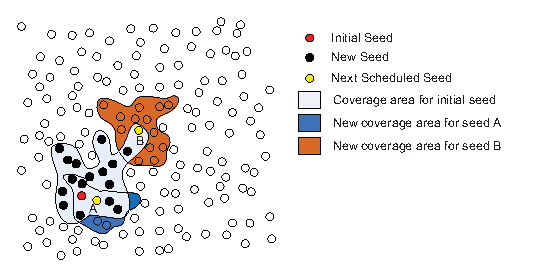
\includegraphics[width=0.5\textwidth]{motivate-example.eps} 
	\caption{A motivating example to demonstrate how seed selection  
		affects the testing efficiency.}\label{motivate-example}
\end{figure}
In order to measure the distances, all test cases should be mapped 
as numerical vectors. 
The mapping can be performed into either the input space or state space. 
Mapping into the input space cannot reflect the real relationship between 
test cases when considering the behavior of the target program. 
As shown in Figure~\ref{distance-illusion}, multiple different 
inputs can steer the program to execute the same path. For example, 
considering the three test cases namely \texttt{A.jpeg}, \texttt{B.jpeg} 
and \texttt{C.jpeg} in this figure, suppose the corresponding contents 
are shown as follows:
\\
\\
\indent\texttt{A.jpeg}: \texttt{$\backslash$xFF$\backslash$xD8$\backslash$xAA$\backslash$xBB$\backslash$xCC$\backslash$xDD}

\texttt{B.jpeg}: \texttt{$\backslash$xFF$\backslash$xD8$\backslash$xDD$\backslash$xCC$\backslash$xBB$\backslash$xAA}

\texttt{C.jpeg}: \texttt{$\backslash$xFE$\backslash$xD8$\backslash$xAA$\backslash$xBB$\backslash$xCC$\backslash$xDD}
\\

\indent If we calculate the \textit{Euclidean Distance} between these 
three files directly in the input space, $ED_{AB}$ will be greater 
than $ED_{AC}$ because there are more different bytes between 
\texttt{A.jpeg} and \texttt{B.jpeg} than that of \texttt{A.jpeg} 
and \texttt{C.jpeg}. This means \texttt{A.jpeg} and \texttt{C.jpeg} 
are more similar (as shown in Figure~\ref{distance-illusion}) from 
the viewpoint of input space. 
However, for most of JPEG process programs, \texttt{A.jpeg} and 
\texttt{B.jpeg} will execute the same path, and \texttt{C.jpeg} 
will execute another path because \texttt{C.jpeg} is an illegal 
JPEG file (bad magic number). So from the viewpoint of the program, 
\texttt{A.jpeg} and \texttt{B.jpeg} are more similar than 
\texttt{A.jpeg} and \texttt{C.jpeg} even though \texttt{A.jpeg} 
and \texttt{C.jpeg} have only one bit difference. 
Since our objective is to maximize the coverage in the state space, 
we choose to map all the test cases as numeric vectors in the state 
space to calculate the distance.

In \cite{wang2015similarity}, all test cases are represented as a branch 
coverage vector $\mathit{V}=(v_1, v_2, \cdots, v_N)$, where $v_i$ is 
0 means the branch is covered, otherwise 1. 
However, different test cases can affect different number of branches, 
so the mapped vectors may have different lengths which cannot be used 
directly for distance calculation. Meanwhile, it will be difficult to 
construct such vectors because obtaining all the branches and listing 
them \textit{orderly} in each vector to avoid obfuscation between 
vectors is nearly impossible for binary programs. 
In AFL \cite{online:afl}, the execution path information of each test 
case is stored as a \emph{Bitmap}. By checking the hit count of this 
bitmap, AFL determines whether some new behaviors are triggered. 
So as this bitmap contains enough information to reflect the 
characteristics of a test case from the viewpoint of the state space, 
we choose the bitmap as our mapped vector to mitigate the costly 
mapping in \cite{wang2015similarity}.

\begin{figure}
	\centering
	
\includegraphics[width=0.3\textwidth]{distance-illusion.eps} 
	\caption{An illusion for distance. The distance from A to B is longer 
		than from A to C in input space, which is opposite in state space 
		because A and B will execute the same path (the red one).}
	\label{distance-illusion}
\end{figure}

Based on the mapped bitmap vectors, the test case queue in the fuzzer 
is enhanced by assigning each test case with weight $W$, where $W$ is 
obtained by calculating the distance between every two test cases. 
Whenever a new seed file is found, the distance between this seed file 
and all the other files in the queue will be measured to calculate $W$. 
Meanwhile, the weight of all the other files in the queue will be 
updated according to the distance to the new seed file. 

Rather than selecting the seed file that has the longest distance to 
the current seed file (which is only a \emph{local optimum solution}), 
our search method selects the file that takes the longest average 
distance from all the other test cases as the next seed file. By 
doing this, we can achieve a \emph{global optimum solution} for this 
searching problem. The weight $W$ for test case $t_k$ is defined 
as follows:

\begin{center}
	$W_k = \displaystyle\frac{1}{N} \sum_{i=0}^{N} D(t_i, t_k)$
\end{center}
where $D(t_i, t_k)$ denotes the distance between $t_i$ and $t_k$ 
based on the three distance measures mentioned before, and $N$ is 
the size of the test case queue. 

We also noticed that even though two test cases have the same $W$ value, 
they may have different power on finding new paths.
This is because path coverage is not the only criteria for testing, 
and other runtime information, such as memory operations, 
can also be leveraged to prioritize test cases. 
So we enhanced the weigh $W$ with memory coverage to achieve 
better prioritization result. The enhanced weight $\hat{W_k}$ for 
test case $t_k$ is defined as the following formula, where $M(t_k)$ 
denotes the number of memory cells that $t_k$ covers in byte.
\begin{center}
	$\hat{W_k} = \displaystyle M(t_k) + \frac{1}{N} \sum_{i=0}^{N} D(t_i, t_k)$
\end{center} 

AFL introduces \textit{Energy} (i.e., mutation times) for each seed based 
on some properties like bitmap coverage, file size, execution time and so on.
For example, a seed with more bitmap coverage will be fuzzed with more times. 
We leveraged the similar idea in our distance based seed selection. 
Based on the enhanced weight, our fuzzer engine assigns each seed with an extra
energy to mutation. That is, a seed in the queue with greater weight will
be fuzzed with more times. By assigning more mutation times for the seed that
may cover more untouched code areas, we increase the probability to trigger
more paths.

\section{Implementation and Evaluation} \label{sec:evaluate}
\prototype is built on top of AFL \cite{online:afl}, a popular 
state-of-the-art genetic fuzzing framework, and the S2E symbolic 
execution platform \cite{chipounov2011s2e}. S2E is a dynamic 
binary analysis platform which utilizes selective symbolic execution 
to analyze whole software stacks at runtime. S2E reuses parts of 
the QEMU virtual machine \cite{bellard2005qemu}, the KLEE symbolic 
execution engine \cite{cadar2008klee} and the LLVM 
toolchains \cite{lattner2004llvm}.

Our implementation consists of two main components, namely
\emph{Symbolic Path Finder (SPF)} and \emph{Seacher}. The \emph{SPF}
component is leveraged to help the fuzzer dive into deeper code areas
that are guarded by complex path constraints. Techniques to handle the
\textit{path explosion} problem raised by symbolic pointers and loops
are implemented inside of \emph{SPF}. The \emph{Searcher} is designed
to assign more mutation energy to the promising seeds based on the weight
value obtained by distance based seed selection method. 
By doing this, the fuzzer will reach previously
untouched more code areas as soon as possible in a given time budget.

In the experimental evaluation part, we address the following 
research questions:
\begin{itemize}
	\setlength{\itemsep}{0pt}
	\item {\textbf{RQ1:} Can \prototype discover more deeper bugs?}
	\item {\textbf{RQ2:} Can distance based seed selection method 
		improve performance of path discovery?}
	\item {\textbf{RQ3:} How does each component contribute to 
		path discovery?}
	\item {\textbf{RQ4:} Did \prototype uncover unreported bugs in real-world binaries?}
\end{itemize}

More specifically, RQ1 investigates the bug discovery ability of 
\prototype on two benchmarks and compares the results with other vulnerability 
detection tools including fuzz testing and symbolic execution.
For RQ2 and RQ3, we choose to use AFL's \textit{unique paths} as performance evaluation criterion since it is a key factor to reflect the 
performance of a path-based program testing tool.
RQ2 evaluates distance based seed selection on several 
real-world programs to see whether our method can discover more 
unique paths than the state-of-the-art fuzzer: AFL. RQ3 evaluates 
the overall unique path discovery performance of \prototype and 
investigates the performance contribution of each isolated 
component (i.e. \textit{SPF} and \textit{Searcher}). RQ4 benchmarks
\prototype on several real-world programs to check whether it can
discover unreported crashes.

Evaluations were conducted on a server equipped
with an Intel Xeon CPU E7-2850@2.0GHz with
10 cores and 64 GB RAM, running Linux Ubuntu 14.04 LTS AMD64.

\subsection{Vulnerability Detection (RQ1)}\label{sec:RQ1}
We evaluated the bug discovery ability of our method with two 
different benchmarks. The first benchmark is a demo program 
which is named as \emph{CommonMB}. 
The second benchmark is \emph{LAVA}, which was released in 2016 
to test different vulnerability discovery tools \cite{dolan2016lava}. 
In the following sections, we are going to introduce the 
two benchmarks, and discuss the testing results of \prototype
as well as other off-the-shelf vulnerability discovery tools 
(AFL, VUzzer, KLEE, and S2E) in detail. AFL and VUzzer are coverage
based fuzzers. VUzzer leverages static analysis to extract comparison
instructions then introduces these information into mutation to improve coverage
\cite{rawat2017vuzzer}. By doing such, VUzzer is good at uncovering magic number
related bugs. KLEE and S2E are both symbolic execution tools. However, KLEE works
in user mode and can only handle compiled LLVM byte code. S2E can deal 
directly with binary executables on full software stack.

\subsubsection{CommonMB}
\noindent The \emph{CommonMB} benchmark is a demo program which contains 
9 different memory error bugs. These bugs can be triggered only when 
feeding the program with specifically crafted input. There are four 
different kinds of functions in this benchmark, i.e., 2 compare-style 
functions, 3 math-style functions, 2 checksum-style functions and 2 
logic-style functions. The compare functions contains bugs that can 
only be triggered when the values of specific parts of the input equal 
to specific constant immediate numbers; the bugs in math functions 
can be triggered when the results of math operation on some specific 
parts of the input equal to specific constant immediate numbers; the 
checksum related bugs can only be triggered when the input data 
successfully goes through the checksum checking points; and the logic 
bugs utilize two simple logical games (maze and semi-sudoku) as the 
constraints for triggering the bugs, which means the bugs can only be 
triggered when the testing engine successfully solves the games. We 
released \emph{CommonMB} benchmark on
\texttt{https://github.com/Epeius/CommonMB.git}.

The bugs in \emph{CommonMB} benchmark represent the common bug conditions 
in real-world programs. For example, compare-style bugs denote the bugs 
that depend on some specific/interesting values in the program; 
checksum-style bugs stands for the bugs whose inputs are well-formatted, 
such as PNG file.
So evaluating a vulnerability detection tool on such a benchmark can 
reflect its ability of discovering bugs in real world programs.

Table~\ref{CommonMB-results-detail} shows the overall results of 
different vulnerability discovery tools as well as \prototype 
with same test environment (10 cores and 12 hours).
% Explain the result like that cmp-style vulnerabiities are easy to find
We can see that all these tools have successfully triggered the 
two compare-style bugs (i.e., \textit{cmp16} and \textit{cmp32}). 
This is because there two functions are in the shallow surface of 
this benchmark and the conditions to trigger the bugs are simpler 
than the others.  

Fuzz testing tool discovered few math-bugs than symbolic execution 
tools. AFL discovered only one bug in MATH (i.e., \textit{add16}).
And it failed to uncover the bug that guarded by complex mathematic operations.
VUzzer failed to detect any bugs in MATH.
All tools that leverage symbolic execution successfully 
triggered all these three bugs since symbolic execution is good at 
solving such corner cases. 

S2E provides function models for basic functions that may fork too 
many states, like \texttt{strcpy}, \texttt{strcat}, \texttt{crc16},
and \texttt{crc32}. Based on these models, S2E and \prototype 
discovered the two bugs that related to checksum successfully 
(note that this does not mean S2E can break these checksum functions). 
Such bugs cannot be uncovered by KLEE. 

Logic-style vulnerabilities are difficult for all tools to uncover 
because the number of states will be infinite in the worse case.
For example, when solving a maze, the possible oscillation between 
two opposite steps (such as step forward and step backward) 
will stop the engine from finding new paths.
With the help of our seed selection method, \prototype assigned 
the seed file with the maximum average distance with more energy to mutate. 
Since this distance metric tries to maximize the memory coverage, 
\prototype successfully triggered the bug after covering all 
the memory access to the maze array. 
% Explain why the sudodu is so hard to touch
However, our \prototype failed to trigger the bug in \textit{sudoku}. 
This is because different seed files of the \textit{sudoku} have no 
significant differences (i.e., no more code/branch and memory coverage), 
which confuses our seed selection method.

Table~\ref{CommonMB-results-detail} also presents the peak memory usage (PMU)
of these tools in KB. From these data, we can see that \prototype consumes
more memory than other four tools, specifically, it brings memory
overhead when compared with vanilla S2E. This is because we run both fuzzer and
symbolic execution in the system. And since \prototype's symbolic execution engine
works on hybrid testing mode which only forks states for only uncovered branches of 
the seed from fuzzer, it brings less memory overhead (1.8\% more).

\begin{table*}[!t]
	\processtable{Evaluation results on \textit{CommonMB} in detail.
		\label{CommonMB-results-detail}}
	{\begin{tabular*}{20pc}{ccccccccccccc}\toprule
			&& \multicolumn{2}{c}{CMP}  & \multicolumn{3}{c}{MATH} & \multicolumn{2}{c}{CHECKSUM} 
			& 	\multicolumn{2}{c}{LOGIC} && \\ 
			Tool & version & cmp16 & cmp32 & add16 & add32 & complex & crc16 & 
			crc32 & maze & sudoku & Total Crashes (\#) & PMU (KB)\\
			\midrule
			AFL 		& 2.52b		& \cmark & \cmark & \cmark & \xmark & \xmark & \xmark & \xmark & \xmark & \xmark & 3 & 4588.0\\
			VUzzer      & 1.0       & \cmark & \cmark & \xmark & \xmark & \xmark & \xmark & \xmark & \xmark & \xmark & 3 & 25702.4\\
			KLEE (Random Searcher)		& 1.4.0		& \cmark & \cmark & \cmark & \cmark & \cmark & \xmark & \xmark & \xmark & \xmark & 5 & 108236.8\\
			S2E			& 2.0		& \cmark & \cmark & \cmark & \cmark & \cmark & \cmark & \cmark & \xmark & \xmark & 7 & 2979048.0\\
			\prototype	& 0.1		& \cmark & \cmark & \cmark & \cmark & \cmark & \cmark & \cmark & \cmark & \xmark & 8 & 3031373.2\\
			\botrule
		\end{tabular*}}{}
	\end{table*}
	
\subsubsection{LAVA Benchmark}
In 2016, Dolan-Gavitt et.al. developed a technique, namely LAVA, to 
automatically inject secure-related bugs into some Linux utilities for 
evaluating the bug-finding tools \cite{dolan2016lava}. These bugs are 
all hard-to-reach memory errors. In the paper of LAVA, the authors describe 
their results on the evaluation of coverage based fuzz testing, an SAT-based 
approach on the benchmark. The LAVA benchmark has two corpus sets, 
i.e., \textit{LAVA-1} and \textit{LAVA-M}.

\textit{LAVA-1} injected 69 different bugs into the \texttt{file} program 
in Linux CoreUtils. There are two types of buffer overflow vulnerabilities 
were injected, one is \emph{Range} and the other one is 
\emph{Knob-and-trigger (KT)}. The Range style bugs are triggered if the 
magic value is in some range and also check the value to determine how much 
to overflow. And in the KT bug, two bytes in the input are checked against 
a magic value to determine if the overflow will happen and another two bytes 
determine how much to overflow. Both the two types of bugs were designed to 
mirror real bug patterns which can be used to evaluate the ability of 
bug-finding tools. Compared \textit{LAVA-1}, which injected only one bug 
in the program, \textit{LAVA-M} injected more than one bug into four 
different programs in CoreUtils that took file input: \texttt{base64}, 
\texttt{md5sum}, \texttt{uniq}, and \texttt{who}, so \textit{LAVA-M} is a 
better benchmark to evaluate the vulnerability discovery tools that are 
designed to work for a long time on programs that may contain multiple bugs.

\begin{table}[!b]
	\processtable{Evaluation results on \textit{LAVA-1}\label{LAVA-1}}
	{\begin{tabular*}{10pc}{@{\extracolsep{\fill}}ccccccc@{\extracolsep{\fill}}}\toprule
			& $2^0$ & $2^7$  & $2^{14}$ & $2^{21}$ & $2^{28}$ & KT \\
			Tool   & 12 bugs & 10 bugs & 11 bugs & 14 bugs & 12 bugs & 10 bugs\\
			\midrule
			FUZZER 					& 0   & 0   & 1    & 11    & 9     & 2  \\
			SES	        			& 1   & 0   & 1    & 3     & 0     & 1  \\
			AFL		    			& 0   & 0   & 0    & 10    & 9     & 1   \\
			VUzzer      			& 0	  & 0   & 0	   & 2     & 1	   & 0   \\
			S2E						& 0   & 0   & 0    & 0     & 0     & 0   \\
			$\prototype_{E}$ 		& 0   & 0   & 0    & 10    & 8     & 0   \\
			$\prototype_{C}$ 		& 0   & 0   & 0    & 9     & 9     & 0   \\
			$\prototype_{J}$ 		& 0   & 0   & 0    & 9     & 8     & 1   \\
			$\prototype$			& 10  & 10  & 11   & 13    & 11    & 7   \\
			\botrule
		\end{tabular*}}{}
	\end{table}
	
Note that since \cite{dolan2016lava} does not make a statement about the details of 
about the tools and experimental setups they evaluated, we took their results
directly into Table~\ref{LAVA-1} and Table~\ref{LAVA-M}. 
Also, because VUzzer runs only on 32-bit system, 
we re-executed VUzzer within a new environment running Linux Ubuntu 14.04 X86 
with the same cores and memory as our experimental setup. Meanwhile, since VUzzer
works on binary mode as well as S2E, \emph{we discard to evaluate KLEE on LAVA benchmark}.

We also list \prototype with different setups in Table~\ref{LAVA-1} and Table~\ref{LAVA-M}. 
Here $\prototype_{*}$ represents \prototype with only \textit{Searcher} disabled, 
where $E,C,J$ denote \textit{Euclidean Distance}, \textit{Cosine Similarity} 
and \textit{Jaccard Index} metrics.

Table~\ref{LAVA-1} summarized the results of bug finding evaluation on 
\textit{LAVA-1} from the LAVA paper as well as some popular off-the-shelf 
tools. The maximum testing time for each bug was 5 hours. 
From this table, we can see that the \textbf{FUZZER} and \textbf{SES} 
mentioned in the paper only found 23 bugs and 6 bugs respectively in total. 
AFL failed to trigger any bugs in smaller ranges ($2^0$, $2^7$ and $2^{14}$) 
but it outperformed VUzzer and S2E in larger ranges. 
VUzzer touched a total of 3 bugs which is less than AFL. 
This is because VUzzer's dynamic taint analysis slowed down
the testing speed but gained little in LAVA-1 since the conditions of triggering
such bugs are not in strictly equality comparison form.

An interesting point is that S2E failed to trigger any bugs in LAVA-1. The reason
is that because LAVA-1 is built on top of \texttt{file} program which contains many
lookup tables by symbolic index, and such code will degrade symbolic execution
to random-like fuzz testing (as shown in Listing~\ref{RE-LCSP}). Meanwhile, 
since S2E works on full system emulation mode and the execution speed is much less 
than fuzz testing in user mode like AFL, it failed to uncover bugs even in larger areas.

\prototype discovered 62 bugs which was much more than the FUZZER and the 
SES tools separately. In particular, we triggered all the bugs in $2^7$ and 
$2^{14}$ ranges. And also found most of the KT bugs (70\%) which cannot be 
touched effectively by the FUZZER and SES tools. By leveraging LCSP algorithm,
\prototype's symbolic execution engine can go through the lookup tables to reach
the bug points, and since the bugs' trigger conditions in LAVA-1 are easy for 
symbolic execution engine, \prototype thus can uncover almost all the bugs in LAVA-1.

We can also derive from Table~\ref{LAVA-1} that the gain of \prototype in LAVA-1 mostly
comes from \textit{SPF} ($\prototype_*$ has the similar performance
with AFL), especially in smaller ranges like $2^0$, $2^7$ and $2^{14}$. 
This is because, even though the fuzzer engine can steer \texttt{file}
program to the bug point, the trigger conditions are complex for $\prototype_*$ to
overcome. 

Table~\ref{LAVA-M} describes the evaluation results on LAVA-M of the FUZZER 
and SES which are mentioned in the LAVA paper. We also listed other popular
tools and \prototype in this table. From this table we can see \prototype
outperformed other tools on this benchmark.

\begin{table}[!b]
	\processtable{Evaluation results on \textit{LAVA-M}\label{LAVA-M}}
	{\begin{tabular*}{20pc}{@{\extracolsep{\fill}}cccccc@{}}\toprule
			& \texttt{base64} & \texttt{md5sum} & \texttt{uniq} & \texttt{who} &   \\
			Tool    & (44 bugs) & (57 bugs) & (28 bugs) & (2136 bugs) &  Total\\
			\midrule
			FUZZER 				& 7  & 2  & 7    & 0   & 16  \\
			SES	        		& 9  & 0  & 0    & 18  & 27  \\
			AFL         		& 2  & 6  & 1    & 3   & 12   \\
			VUzzer				& 14 & 1* & 24   & 103 & 142 \\
			S2E         		& 1  & 0  & 0    & 2   & 4   \\
			$\prototype_{E}$	& 1  & 6  & 1    & 4   & 12 \\
			$\prototype_{C}$	& 2  & 4  & 1    & 4   & 11 \\
			$\prototype_{J}$	& 1  & 4  & 1    & 3   & 9 \\
			$\prototype$		& 37 & 29 & 28   & 203 & 297 \\
			\botrule
		\end{tabular*}}{}
	\end{table}

As mentioned in the LAVA paper, SES cannot find any bugs in \texttt{uniq} and 
\texttt{md5sum}. And the reasons are the control flow is too unconstrained in 
\texttt{uniq} and SES failed to execute any code past the first instance of 
the hash function. 
VUzzer outperformed AFL in \texttt{base64}, \texttt{uniq} and \texttt{who}, 
but it failed to trigger more bugs than AFL in \texttt{md5sum}. 
This is because it failed to get through the first crash to parse more of any input \cite{rawat2017vuzzer}, whereas \prototype successfully triggered 29 bugs in 
\texttt{md5sum}.

Similar to LAVA-1, the bug points in LAVA-M are also easy-to-reach. This is why
$\prototype_*$ bring little performance improvement when compared with AFL. However,
since \textit{SPF} leverages symbolic execution to solve the bug conditions, more
bugs are exposed.

Since the role of the fuzzer (specifically, \textit{Searcher}) in hybrid testing 
is to find as many code areas as possible,
we devised more experiments
to illustrate the coverage performance of distance based seed selection method
in \ref{sec:RQ2} and \ref{sec:RQ3}.

\subsection{Coverage Performance (RQ2)}\label{sec:RQ2}
Our benchmark for coverage performance evaluation consists of 8 real-world binary 
programs, and the input file formats of our benchmark cover a range of types such 
as executables, images, archives and network packets.

To set the baseline of coverage performance, we utilized the state-of-the-art 
coverage based fuzzer AFL \cite{online:afl} and configured it to run under 
\textit{binary-testing} (i.e., option `-Q' is turned on) mode with one 
single work node.
We collected and compared \textbf{the number of unique paths} found by 
AFL and our distance based seed selection method.
Then we select the most effective distance metric for 
subsection~\ref{sec:RQ3}.
All the evaluations lasted for 24 hours.

The evaluation results were shown in Table~\ref{PD-8samples}. We have 
investigated the three distance measures mentioned before (i.e., EU, CS, 
and JI) as well as vanilla AFL (Order).
From this table, we can see that by assigning more mutation energy to promising
seeds, the fuzzer can touch more unique paths in average.
More clearly, Figure~\ref{path-detail}(a) shows the normalized unique 
paths to vanilla AFL for these 8 programs 
based on the results in Table~\ref{PD-8samples}.
\begin{table}[!b]
\processtable{Number of unique paths discoverd for 8 sample programs\label{PD-8samples}}
{\begin{tabular*}{20pc}{@{\extracolsep{\fill}}lrrrr@{}}\toprule
		Program  & Order\# & EU\# & CS\# & JI\# \\
		\midrule
		\texttt{readelf}  &    2753 & 4595 & 5314 & 5062 \\
		\texttt{djpeg }  &    2802 & 3020 & 4198 & 3390 \\
		\texttt{objdump} &    1755 & 2200 & 2960 & 2133 \\
		\texttt{gzip }  &    1440 & 1564 & 1754 & 1588 \\
		\texttt{ffmpeg}  &    5022 & 5993 & 6181 & 5801 \\
		\texttt{tcpdump}  &    3399 & 3673 & 4267 & 2950 \\
		\texttt{capstone} &    5626 & 6008 & 6066 & 5873 \\
		\texttt{gif2png}  &     912 &  981 & 1100 &  997 \\ 
		\botrule
	\end{tabular*}}{}
\end{table}


From Figure~\ref{path-detail}(a), we can see that both EU and CS metrics 
can outperform vanilla AFL on discovering unique paths for all programs 
in our benchmark. However, the average performance gain of EU is 
lowers than CS metric. 
Compared with the other two distance measures, JI is the most unstable 
strategy which discover more unique paths for some programs, like 
\texttt{readelf}, \texttt{djpeg}, but also brings performance overhead 
for some others, such as \texttt{tcpdump}.

An interesting point from Figure~\ref{path-detail}(a) is that, for 
\texttt{capstone}, the performance gain of CS metric is not as 
significant as the other 7 programs (found only 8\% more paths 
than vanilla AFL).
This is because, in our experiment, the input of \texttt{captone} 
was only plain texture file with some assembly code in it. Such kind 
of input is not as well formatted as other inputs like ELF, JPEG, 
CAP and so on. 
So modifying any parts of the input may have same probability to
trigger new behaviors which means each seed file in the queue 
will have nearly the same power to cover new code areas. This 
also demonstrates that our seed prioritization method will gain 
more performance for well-formatted inputs.

To demonstrate the path discovery speed along with test time, 
we selected four representative programs, i.e., \texttt{readelf}, 
\texttt{ffmpeg}, \texttt{objdump}, and \texttt{tcpdump}, in our 
benchmark and collected the number of unique paths every two 
hours (the number for each program is normalized to the 
maximum to make this figure more clear).
The results are shown in Figure~\ref{path-detail}(b), where 
the x-axis indicates the test time in hours; while the y-axis 
shows the normalized unique number of paths triggered 
by each strategy.
As shown in Figure~\ref{path-detail}(b), both CS and EU performed 
consistently better than orderly during all the 24 hours.
More specifically, EU performed better than CS in the first 
several hours, and then CS outperformed EU in the following test time.
While JI performed well in \texttt{readelf}, \texttt{ffmpeg} and 
\texttt{objdump}, but it failed to improve the performance in 
\texttt{tcpdump} after testing for 8 hours.

Especially for \texttt{ffmpeg}, we can see that in the first 4 hours, 
all of these four selection strategies achieved the same 
performance on discovering unique paths. However, vanilla AFL 
failed to trigger more unique paths during 4$\sim$18 
hours before it started to find new paths again.
This is because the mutation areas of seeds that processed 
during 4$\sim$18 hours are overlapped with each other 
(as shown in Figure~\ref{motivate-example}), which will not 
contribute any new paths. However, our distance based 
seed selection strategy can consistently trigger new paths 
during 24 hours as shown in this figure.

Based on the results, we can obtain that our distance based seed 
selection strategy (especially CS metric) can achieve 
higher performance than vanilla AFL. So we selected CS metric as 
our selection strategy in the following evaluation section.

\begin{figure}[!t]
	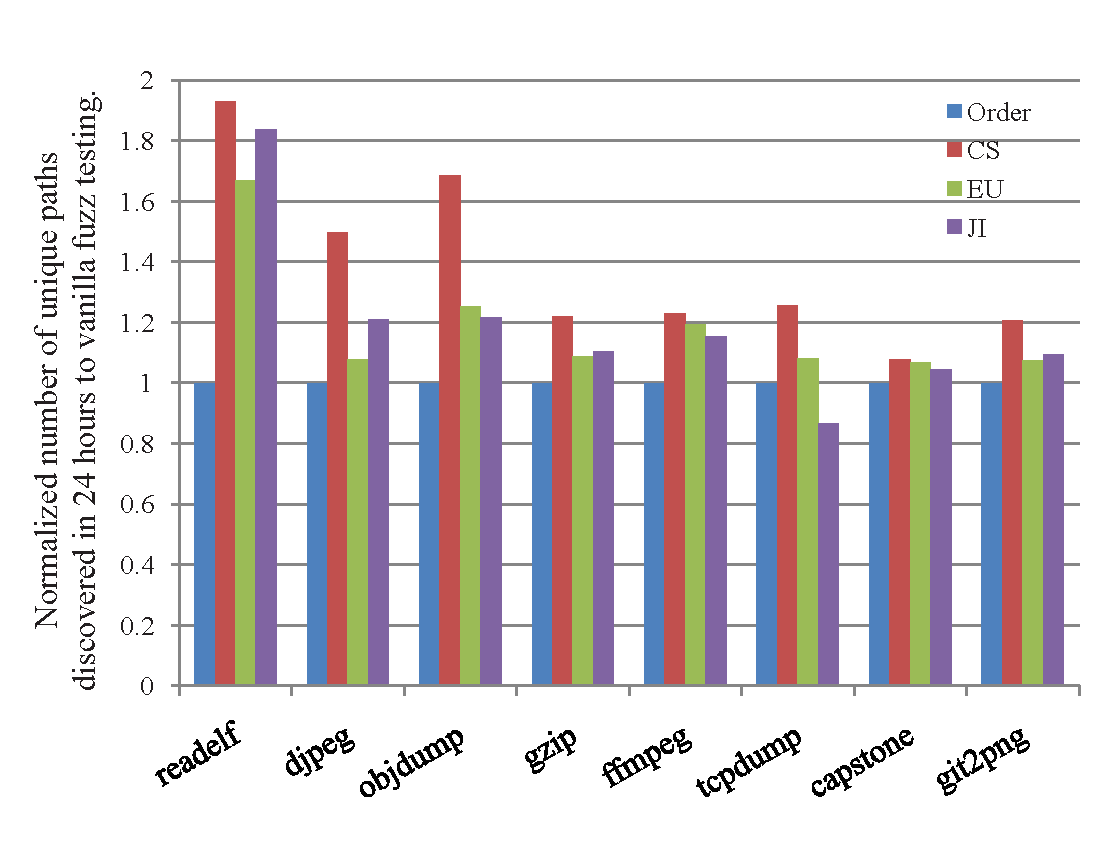
\includegraphics[width=0.45\textwidth, trim={0.2cm 0.4cm 0cm 0cm}, clip]
	{path-discovery.eps}
	\figfooter{(a)}{Normalized number of unique paths for these 
		four selection strategies to vanilla fuzz testing (i.e., \textit{Order}) }
	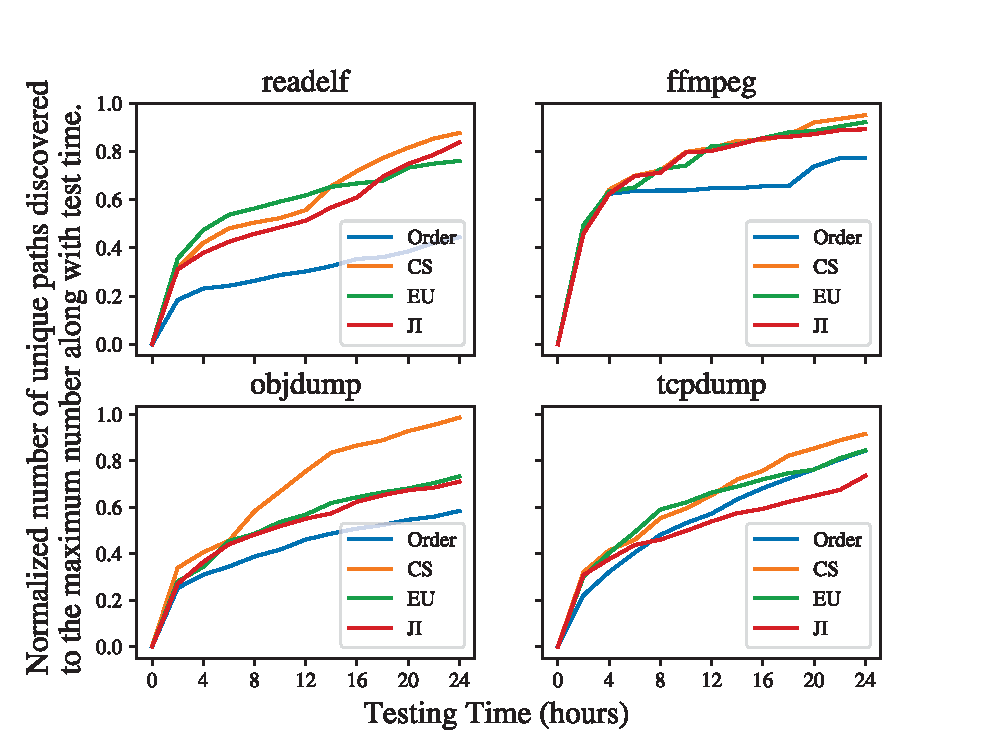
\includegraphics[width=0.45\textwidth, trim={0.15cm 0.1cm 1.5cm 0.8cm}, clip]
	{path-time-detail.eps} 
	\figfooter{(b)}{Path discovery details along with 24 hours for 
		four sample programs.}\label{fig1}
	\caption{Path discovery results for different seed selection strategies.}
	\label{path-detail}
\end{figure} 
		
\subsection{Improvement Detail for Each Component (RQ3)} \label{sec:RQ3}
In order to evaluate the contribution of each component on finding 
unique paths, we conducted four experiments (i.e., vanilla AFL fuzz testing, 
symbolic execution assisted hybrid testing (\textit{SEHT}), SEHT with \textit{SPF}, 
SEHT with \textit{SPF\&Searcher}) and compared their results in 24 hours.

In our experiments, since Driller \cite{stephens2016driller} does not support 
real-world binary programs very well now (many library functions and system 
calls are not modeled), we reimplemented the mechanism of Driller within 
S2E to collect the results for SEHT. And based on the results of 
subsection~\ref{sec:RQ2}, our searcher employs \emph{cosine similarity} 
as the distance metric.

Figure~\ref{path-overall-rsults} summarizes the results of how each 
component contribution to the performance improvement. Compared with 
vanilla fuzz testing, symbolic execution assisted hybrid testing can 
discover 11.88\% more unique paths in average. For example, this 
improvement reaches the highest figure of 42.79\% for \texttt{readelf}. 
However, the performance gain is lower than 20\% for the other 7 programs. 
Specifically, SEHT triggered only 1.32\% more unique paths 
than vanilla fuzz testing for \texttt{gif2png}. This is because the 
symbolic execution engine does not support to handle float number 
operation. After employing \textit{SPF} which handles symbolic pointers 
and symbolic loops, 7.22\% more unique paths touched by SEHT with \textit{SPF}
than SEHT in average. We can see from this figure that 
the performance of SEHT is highly improved by \textit{SPF} 
for \texttt{readelf} and \texttt{objdump} (18.02\% and 22.62\% respectively).

This improvement can be continually augmented by cooperating with CS 
searcher (SEHT with \textit{SPF} and CS \textit{Searcher}). For example, the number 
of unique paths discovered by SEHT is increased by 
49.57\% for \texttt{objdump}. In average, the performance of SEHT 
is improved by 24.44\% after introducing \textit{SPF} and CS \textit{Searcher}. From an 
overall viewpoint, \prototype can discover 43.49\% more unique paths 
than vanilla AFL fuzz testing for our benchmark. This improvement is 
because that seeds file with longest distance from already-explored 
spaces have higher likelihood to trigger more fresh branches/paths, 
so solving such seed files earlier by symbolic execution can find more 
fresh seed files than other files. \\


Above all, we can obtain that \textit{Searcher} contributes larger 
proportion of contribution to unique path discovery than \textit{SPF}. 
However, this does not mean the contribution of \textit{SPF} is 
negligible. By integrating \textit{SPF} component (i.e., \textit{LCSP} 
and \textit{SLB}), the symbolic execution engine can dive into deeper 
code areas to solve \textit{complex branch conditions} to help fuzzer 
find more fresh paths and discover more hard-to-reach vulnerabilities
(as shown in \ref{sec:RQ1}).
		
		
\begin{figure}
	\begin{center}
		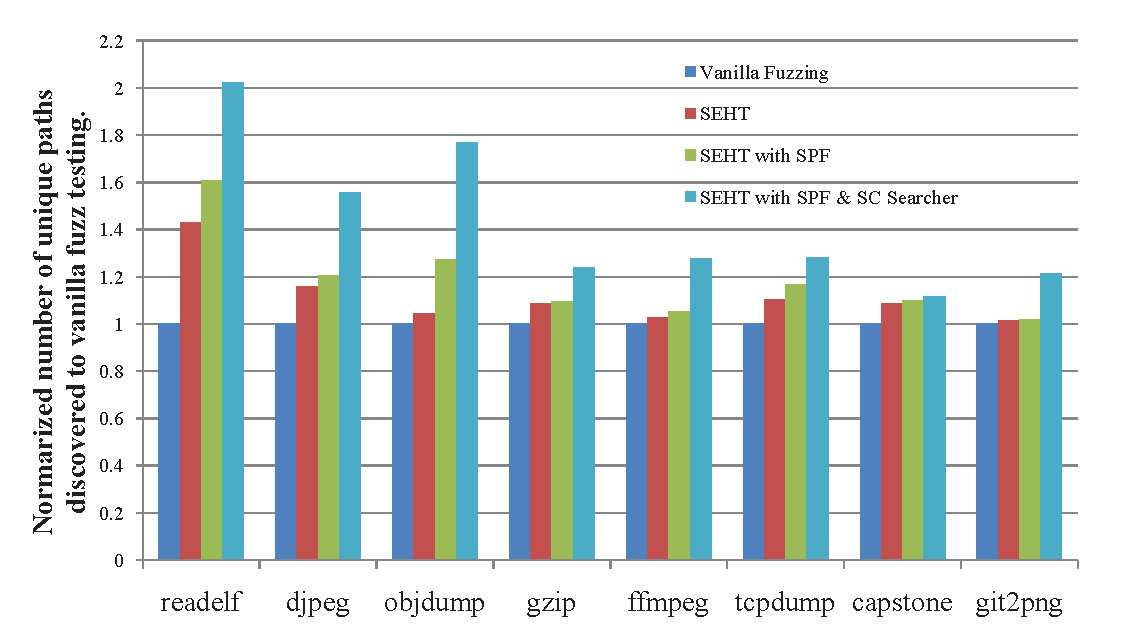
\includegraphics[width=0.5\textwidth]{path-discovery-SPF-CS-all.eps} 
		\caption{Normalized number of unique paths discovered for each component to vanilla fuzz testing.}\label{path-overall-rsults}
	\end{center}
\end{figure}

\subsection{Unknown Crashes Discovered in Real-World Binaries (RQ4)} \label{sec:RQ4}
We selected several real world programs to evaluate the ability of unknown bug 
discovery of our system. The input types of this dataset cover ELF binary, 
multi-media, image, and packet capture. In order to demonstrate the efficiency 
of our system, we also compared our results with AFL and VUzzer. We ran each
program under the same testing environment with one fuzzing node for 24 hours. 

Table~\ref{zero-days} shows the results of our testing. 
From the table we can see that during 24 hours, \prototype triggered 403 
unique crashes in the dataset which outperformed vanilla AFL (181 unique crashes) 
and VUzzer (192 unique crashes). 
We can also derive from this table that our method gains little for \texttt{mp3gain} 
and \texttt{madplay}. This is because our symbolic execution engine does not support 
the float number operation when handing MPEG/WAV format (for example, all the 
writing operation to \texttt{XMM} registers will be concretized). This concretization 
lost some interesting paths and made less contribution to bug finding(only 2 more 
bugs for \texttt{mp3gain} and 1 more bug for \texttt{madplay}). 
This also explains why VUzzer found more bugs in \texttt{mp3gain} 
than \prototype. 
It is interesting that AFL detected 15 more bugs in \texttt{elfparser} than VUzzer. 
This is because the fork server method leveraged in AFL enables the fuzzer can 
execute 51.6x more test cases than VUzzer in the same time, which can also increase 
the probability of finding bugs.
		
\begin{table*}[!t]
	\processtable{Performance of our method VS. AFL \& VUzzer on unknown crashes.\label{zero-days}}
	{\begin{tabular}{lccccccc}\toprule
			& & \multicolumn{2}{c}{\prototype} & \multicolumn{2}{c}{AFL} & \multicolumn{2}{c}{VUzzer}\\
			Program & Input Type & Crashes (\#) & Executed (\#)& 
			Crashes (\#) & Executed  (\#) & Crashes (\#) & Executed (\#) \\
			\midrule
			\texttt{elfparser}  & ELF	& 60 &   1.1M & 48   & 1.0M   & 33 & 19.0K    \\
			\texttt{distorm}    & ELF    & 13 &   16.2M   & 0   & 15.7M    & 3 & 93.1K    \\
			\texttt{mp3gain}*   & MPEG	& 43 &   11.3M  & 41  &  11.7M   & 46 &  79.3K  \\
			\texttt{madplay}*   & WAV	& 55 &   15.9M  & 54  & 14.3M    & 52 & 88.7K   \\
			\texttt{optipng}    & PNG    & 49 &   9.5M & 15  &  10.1M   & 32 & 54.1K   \\
			\texttt{tstat}      & PCAP   & 183&   6.4M & 23 &  6.2M   & 26 & 48.5K   \\
			\midrule
			Total      &        & 403   &  & 181 &  & 192 &\\
			\botrule
		\end{tabular}}{}
	\end{table*}


\section{Limitations and Discussion} \label{sec:discussion}
Our method is built on top of coverage based fuzz testing and dynamic 
symbolic execution, where we have introduced distance based seed search 
strategy, symbolic loop bucket, and lazy symbolic pointer. While an 
improvement, there are still some drawbacks to our method. This section 
discusses these limitations and take a future look at 
the vulnerability discovery.

\subsection{Limitations}

\noindent\textit{\textbf{Distance Measurement:}} Our seed selection 
strategy leverages three well-known distance measures, i.e., 
Euclidean Distance, Cosine Similarity and Jaccard Index. Also, 
we have evaluated these three measures and compared the results 
with no search strategy. In the future, we hope to investigate 
other distance metrics (e.g.\ hamming distance, N-gram distance, 
etc.) to find a better measurement for different execution paths 
(or different seed inputs). 

\noindent\textit{\textbf{Plain Input Format:}} Programs that accept 
input with no specific format cannot gain performance improvement 
from our distance based seed selection method. As shown in 
Figure~\ref{path-detail}(a), all of these three distance based 
selection strategies failed to trigger more new behaviors for 
\texttt{capstone} which accepts the plain texture file as input. 

\noindent\textit{\textbf{Float Point Operation:}} The dynamic 
symbolic execution engine we depend on will concretize symbolic 
write operations to \texttt{XMM} registers, which will lose some 
interesting paths when handling float point arithmetic operations. 
For example, the \emph{Floating-point Number} benchmark in \cite{xu2017benchmarking}
makes an obstacle for KLEE to solve.
This problem also happens for most of the image processing programs. 
So the dynamic symbolic execution engine should be upgraded to 
support float point arithmetic operations to handle 
these types of programs.

\subsection{Future Work on Vulnerability Detection}
This section will briefly propose some possible future 
research areas in vulnerability detection.

\subsubsection{Binary Transformations}
Dynamic symbolic execution still faces scalability problem 
when considering the size and complexity of modern software. 
Compiler optimizations can have a large impact on dynamic 
symbolic execution's effectiveness. 
In 2013, J. Wagner et, al. proposed a new compiler option 
\textsc{-Overify} to generate code optimized specifically 
for verification tools. Their experiments' results show that 
\textsc{-Overify} can reduce verification time by up to 
95x for GNU Coreutils \cite{wagner2013overify}. As discussed 
in \cite{Cadar:2015:TPT}, LLVM compiler's \texttt{-O0} flag 
can contribute different paths from flag \texttt{-O2} (which 
contributes 1024 and 2 paths respectively for its sample code).
Cadar claims that one should treat program transformations as 
first-class ingredients of scalable symbolic execution, 
alongside widely-accepted aspects such as search heuristics 
and constraint solving optimizations \cite{Cadar:2015:TPT}. 

With this insight, we propose that in the future, binary executables 
should be pre-processed to transform \textit{testing-expensive} 
code structures to \textit{testing-cheap} ones. For example, transforming
a long string comparison instruction to several isolated byte comparison
instructions will improve the performance of fuzz testing.
Similar to \cite{wagner2015high}, the binary pre-processing stage 
should recognize which code areas are the testing ``hot spot'' and 
remove/transform them to avoiding getting stuck in such areas.
These transformations can either be semantic-preserving or 
semantic-altering transformations. The key research problem is how 
to perform these transformations on binary level, since most 
high level program information is lost during compilation. 
On possible solution to achieve such transformations is to lift 
binary code into intermediate expression such as LLVM byte code, 
then perform more analysis to recover program information such 
as control flow graph, data dependency, and control dependency. 

\subsubsection{Finding Bugs with Machine Learning}
Many research papers treat the vulnerability detection with dynamic 
symbolic execution and fuzz testing as a search problem.
Since the search space of modern software can be vast, exhaustive 
exploration of this space is currently impossible.
Reducing the search space may lead to better coverage.
However, this may miss interesting sub-spaces where contain vulnerabilities. 
In order to find deeper bugs when reducing the search space, 
one has to locate \textit{secure-sensitive code areas} based on 
static analysis, and then uses search heuristics to guide 
the program exercise these areas.
Since each type of vulnerability has its own unique 
characteristic \cite{MBishop:ATBOC, wang2009intscope, wang2010ricb}, 
some researchers have attempted to use machine learning to 
automatically extract such characteristics in source code, and 
then predict potential vulnerabilities \cite{VCCFinder, Yamaguchi:2011:VEA}.

In 2016, Grieco et, al. proposed a binary software vulnerability 
predict tool \textsc{VDiscover} as well as a public dataset that 
collects raw analyzed data \cite{Grieco:2016:TLV}. 
They ``managed to predict with reasonable accuracy which programs 
contained dangerous memory corruptions'' \cite{Grieco:2016:TLV}.
Based on such work, we propose that in the future, machine learning 
could be ported to binary software vulnerability detection by 
cooperating with guided testing techniques. Since machine learning 
can raise many false positives, one can leverage guided dynamic 
symbolic execution to mitigate the false positives and verify the 
existence of potential vulnerabilities.

\section{Related Work} \label{sec:related}
% Related Work.tex
We have presented the major advantages of our method in the previous sections and compared our system with some state-of-the-art vulnerability discovery tools. In this section, we present the techniques that related to our method.

\noindent\textit{\textbf{Similarity Distance in Regression Testing:}}
Similarity based algorithms have previously been leveraged in regression test case prioritization \cite{wang2015similarity, zhang2012simfuzz, jones2003test}. Test case prioritization is a hot research topic in regression testing research, which tries to optimum mutation schedule based on a specific prioritization criterion. Rothermel et, al. proposed fine-grained prioritization strategy based on the instruction coverage and branch coverage \cite{rothermel2001prioritizing}. Then Elbaum et, al. concentrated on function level coverage and they proved that this kind of coarse-grained instrumentation which can reduce the execution overhead but will lose some prioritization performance \cite{elbaum2001incorporating}. Krishna et al. utilized Levenshtein distance as the criterion of prioritization \cite{krishnamoorthi2009factor}. Rather than using an ordered branch sequence to present the path in \cite{wang2015similarity}, we represented the execution path by using the bitmap in AFL, which is more practical and efficiency.

\noindent\textit{\textbf{Taint Analysis based Fuzz Testing:}}
Taint analysis based fuzz testing uses dynamic taint analysis (DTA) to locate regions of seed input that affect the execution path. BuzzFuzz uses DTA to automatically locate regions of original seed input files that influence values used at key program attack points, and then automatically generates new fuzzed test input files by fuzzing these identified regions of the original seed input files \cite{ganesh2009taint}. TaintScope is a directed fuzzing tool working at X86 binary level. Based on fine-grained DTA, TaintScope identifies which bytes in a well-formed input are used in security-sensitive operations (e.g., invoking system/library calls) and then focuses on modifying such bytes. And TaintScope is also capable of bypassing checksums via control flow alteration \cite{wang2010taintscope}. Dowser is a guided fuzzer that combines static analysis, DTA, and symbolic execution to find buffer overflow vulnerabilities deep in a program’s logic, and it ranks pointer dereference instructions according to their complexity, and then uses symbolic execution to zoom in on the most interesting operation \cite{haller2013dowsing}.

\noindent\textit{\textbf{Dealing with Symbolic Pointers:}}
The symbolic pointer problem occurs when the program dereferences a symbolic address. 
Previous work on symbolic execution deals with this problem by leveraging the full symbolic memory model \cite{song2008bitblaze, thakur2010directed, brumley2011bap, trtik2014symbolic}. Under this model, if an instruction reads/writes to a symbolic address, then each possible value of this address will fork a corresponding state so that all possible paths can be exercised.
As previously discussed, forking state for each possible value will quickly cause path explosion. 
In 2014, Mayhem \cite{cha2012unleashing} introduced a partial memory model to ease the scalability problem inherit in the full symbolic memory model. 
In the partial memory model, states are only forked when reading a symbolic pointer.
A write operation causes the symbolic pointer to be concretized.
This can reduce the number of forked states, but a high number of read operations may still cause path explosion.
Our LCSP method takes advantages of S2E's lazy forking to postpones the path explosion problem to a later moment. 
LCSP can also improve code coverage by solving the pending states from lazy forking on demand.
Recently, \textsc{MemSight} \cite{Coppa:2017:RPR:3155562.3155638} introduces a new approach 
to symbolic memory that reduces the need for concretization but still can explore more states.
It leverages stage merging \cite{Avgerinos:2014:ESE:2568225.2568293} to compact symbolic 
pointer read operations. Some optimizations are introduced to deal with performance issues
in \textsc{MemSight}, e.g., it constraints the range of symbolic pointer to a certain interval by leveraging SMT solver, which we also used in \prototype. It also proposed  a
memory-wise \emph{paged interval tree} to enable better memory space usage. The experimental
results compared with Angr show \textsc{MemSight} enables the exploration
of states unreachable by previous techniques. Since we are dealing with the symbolic pointer
problem in hybrid testing of real-world binaries, which currently Angr cannot support very
well now (e.g., complex library function model problem), we will investigate more about \textsc{MemSight} in the near future to adopt its advantages in hybrid testing.

\noindent\textit{\textbf{Hybrid Testing Method:}}
As mentioned before, our method is not the first tool to combine fuzz testing and symbolic execution. Hybrid Fuzz Testing uses symbolic execution to discover frontier nodes that represent unique paths in the program \cite{pak2012hybrid}. After collecting as many frontier nodes as possible under a user-specifiable resource constraint, it transits to fuzz the program with random inputs. This tool focuses on binaries but only performs the one-time transition between symbolic execution and fuzz testing. Hybrid Concolic Testing implements multiple transitions between symbolic execution and fuzz testing \cite{majumdar2007hybrid}. But because it is built on top of CUTE, a source code oriented testing tool, so hybrid concolic testing still cannot be deployed on binary testing directly \cite{sen2005cute}. Driller is an up-to-date hybrid testing tool that leverages fuzz testing and concolic execution in a complementary manner to find deeper bugs \cite{stephens2016driller}. It is more practice when compared with previous hybrid tools. Some other tools try to make full use of symbolic execution to maximize the code coverage, they collect symbolic constraints placed on each input and then negating these constraints to generate a new test case that will take another uncovered path, such as SAGE \cite{godefroid2012sage}, Dowser \cite{haller2013dowsing}, FuzzWin \cite{online:fuzzwin} etc. However, as these tools execute each input in the symbolic mode which determines that they have to face the path explosion problem. 

\section{Conclusion} \label{sec:conclusion}
In this paper, we focused on improving the performance of hybrid 
testing method built on coverage based fuzz testing and dynamic 
symbolic execution. We proposed a novel method, lazy concretization, 
to deal with symbolic pointers. We found that this method mitigates 
the path explosion problem and improves code coverage. We also introduced 
the loop bucket optimization in order to avoid generating too many 
states in symbolic loops. In order to deal with the large size of 
the seed queue in hybrid testing, we presented a distance-based seed 
selection method to achieve more coverage when testing time is limited. 
This criteria of selection method is built on top of runtime information 
(i.e, path and memory information). The evaluation of \prototype 
on several benchmarks demonstrates that our method can discover more 
unique paths than vanilla fuzz testing and finds more bugs compared 
with other off-the-shelf vulnerability analysis tools.

\bibliography{biblio.bib}
\bibliographystyle{plain}

\vfill\pagebreak

\end{document}
